\section{Evaluation}

In this paper we have also empirically evaluated how effective deadlock exception can be.

We had two implementations of reentrant locks where one of them was the one provided by
Java's \emph{ReentrantLock} and the other was that lock modified to throw exception when
a deadlock happened. Later we may refer to our implementation as \emph{LockA} and the default
one as \emph{LockB}.

In order to compare each implementation, we conducted
a controlled experiment where students had to run two specific programs with deadlocks
easy to reproduce while collecting the time taken to identify the problem. They also
had to provide a clear explanation of the problem, describing what the problem is, which method
calls were involved on it and a description of how it happens, so we could measure answer precision.

\subsection{Experiment Definition}

The goal of our experiment was to analyze the process of bug identification with the purpose of evaluating efficiency of deadlock exceptions,
in respect to the time spent in order to identify the problem and the accuracy of the descriptions provided by the students. We can define two
research questions we want to answer in this experiment:

{\bf RQ1.} Is the time spent to identify the bug reduced for implementation with deadlock exception when compared to the default implementation?

The metric we watched to answer this question was the time, in seconds, to finish each question in the test.

{\bf RQ2.} Is the accuracy of bug description improved for implementation with deadlock exception when compared to the default one?

Each question's answer was splitted in a few criterias and each criteria was rated between 0 and 1, where 0 means not present, 0.5 means partially present and 1 for fully present:

\begin{description}
\item[A.] Correctly classified problem as deadlock.
\item[B.] Classified problem as different from deadlock.
\item[C.] Correctly identified method calls involved in the deadlock.
\item[D.] Correctly identified locks involved in the deadlock. 
\item[E.] Pointed unrelated methods as part of the deadlock.
\end{description}

To answer this research question, we have classified students answers as either correct or incorrect. Correct answers should respect the following equation:

\begin{equation}
  (A - B) + C \geq 1.5 \;
\end{equation}

We decided to rule out criterias \emph{D} and \emph{E} because the problem statement was not clear they should describe which locks were involved in the deadlock; also, our deadlock implementation at that time could only guarantee at least one deadlock exception to be thrown thus affecting at least one method. In other words, this equation means that a correct answer is whenever the bug was described as deadlock and at least one of the methods involved were identified.

\subsection{Experiment Planning}

In order to evaluate each element described on the previous section, we describe the following statistical hypotheses.

\emph{1) Hypothesis:} To answer \emph{RQ1} regarding the time spent to identify a bug in the code:

\begin{equation}
  H_{0} : \mu_{TimeLockA} \geq \mu_{TimeLockB}
\end{equation}
\begin{equation}
  H_{1} : \mu_{TimeLockA} < \mu_{TimeLockB}
\end{equation}

And to answer \emph{RQ2} regarding accuracy of answers:

\begin{equation}
  H_{0} : \mu_{CorrectAnswersLockA} \leq \mu_{CorrectAnswersLockB}
\end{equation}
\begin{equation}
  H_{1} : \mu_{CorrectAnswersLockA} > \mu_{CorrectAnswersLockB}
\end{equation}

\emph{2) Design, Instrumentation and Subjects:} For this empirical experiment, we have chosen two metrics: time to answer a question and number of correct answers.

In order to prevent \emph{bias}, we needed to control a few factors during the experiment execution. The first factor was the selection of subjects to participate on this experiment, as different background knowledge could potentially influence chosen metrics. The second factor we had to control was the complexity of programs that each subject. Complexity we define as the amount of files in the program, number of threads and number of locks to analyze; as we assumed that easier programs could have little or no benefit from deadlock exceptions, we wanted to have one program that we considered easy to identify the problem and another that was way more complex, spread in more files and classes, thus reflecting a more realistic case. We provided implementations of each program using either \emph{LockA} or \emph{LockB}: the two possible treatments that we want to compare.

We decided to use Latin Square Design to control these two factors mentioned earlier: subjects and program complexity factors. Since we had N subjects, 2 programs and 2 possible treatments, we disposed subjects in rows and programs in columns of latin squares, randomly assigning in each cell of the square a treatment that could be \emph{LockA} or \emph{LockB}, but also guaranteeing that for any given row or column in this square, each treatment appears only once (see Table 1). Consequently, we have replication, local control and randomization which are the three principles of experiment design. % TODO: add ref source %

\begin{table}
\begin{center}
\caption{Latin Square design}
\begin{tabular}{|l|l|l|}
\hline
 & Program 1 & Program 2\\
\hline
Subject 1 & LockA & LockB\\
Subject 2 & LockB & LockA\\
\hline
\end{tabular}
\end{center}
\end{table}

We wrote two programs with different complexity which were presented in the same order for all subjects. The first program, known as \emph{Bank}, contained 4 classes spread in 4 files, 3 threads, 3 explicit locks, and 82 lines of code in average. The second program, known as \emph{Eclipse} had 15 classes spread in 11 files, 4 threads, 5 explicit locks, and 40 lines of code in average. We expected the first program to be easier to identify the deadlock because it contained fewer classes and files. Each program could use either \emph{LockA} or \emph{LockB} but we randomly assigned a group to each student so that if they fall into group A, they would start with \emph{LockA} in the first question, but change to \emph{LockB} on the second question; or if they fall in group B, they they would start with \emph{LockB} and switch to \emph{LockA} in the second question. We randomly paired subjects in tuples composed of one subject in group A and another subject of group B, then we created latin squares for each one of these pairs, where any remainders were discarded.

% insert each program description here, where the deadlock was, etc. in the end, point to where the source for each pdf is %

We have repeated this experiment for two groups of students with different backgrounds. The first group consisted of undergraduate students attending Programming Language Paradigms course. They had classes about concurrent programming, including exercises in Java using ReentrantLock where deadlocks and other concurrent bugs should be avoided; however, these students were not experienced in this area. The second group consisted of graduate students enrolled in master's degree or PhD program attending Parallel Programming course where they had classes about advanced concepts of parallel programming and had a lot of practical exercises, including implementing their own lock; thus, they were expected to have a lot of experience. We did a survey with the second group to understand their background even further (see charts below) at the end of the experiment.

% TODO: insert chart with survey results

\emph{3) Metrics Collection:} Each one should start the experiment with the first question containing \emph{Program 1} and once they finish to provide an answer, they should request for the second question. At that point, we collect and place a timestamp in their answer. Once they finish the second question containing \emph{Program 2}, then they should again give us a notice so we can leave a new timestamp. We have used these timestamps to measure how long they took to finish each question. We have started this experiment with a time limit for each question of 60 minutes each. However, during the test we realized it could not be sufficient for all students so we expanded to 90 minutes each.

The timestamp was written by students conducting the experiment based on a counter we projected on the laboratory wall in real time. In a few circunstances the subject could write the timestamp when they finish, but we have double checked the value at the time we collected their answer, overwriting in case they did any mistake.

\subsection{Experiment Operation}

We executed this experiment in two different days. In the first day we did it with undergraduate students in replacement of their default exam, so their participation was obligatory but we disclaimed they could optionally leave a comment if they did not want to take part in this research, so we would not use their data. Fortunately no one chose to not participate. In the second day, we did it with graduate students after the last class of Parallel Programming course and it was optional. In total, 31 students participated on the first day and 16 students participated on the second day, but we had to discard 2 students data because they arrived late and they had to leave early.

On the first day we started with a time frame of 2 hours for the whole experiment, so we decided to set a deadline for each question and put a time limit of 1 hour each. Later we expanded the time limit to 1 hour 30 minutes for each question. On the second day we decided to stick with 1 hour each because there was no demand to extend it.

\subsection{Experiment Results}

We can split the experiment analysis in two parts:

\emph{1) Time Analysis:} Time analysis was conducted with R Statistical Software using the inputs extracted from each experimentation day. We used the linear model described in Figure 1 that considers the effect of different factors on the response variable.

Initially, we've plotted the box-plot graphic shown in Figure 2 and we can see that answers with \emph{LockB} involved took more time to complete, but suddenly stop to grow not far from where \emph{LockA} reaches its peak. If there was no time limit on each question, we believe that \emph{LockB} times would show a much higher range.

Then we've run the Box-Cox transformation - which is a power transformation - to reduce anomalies such as non-addivity and non-normality, obtaining the curve in Figure 3. As the value of $\lambda$ at the maximum point in the curve is not approximately 1, we should apply the transformation; that is, $Y_{lijk}$ should be powered to that $\lambda$ on our regression model. Running the same analysis again with the transformed model, we obtain the curve shown in Figure 4.

\begin{figure}
\begin{center}
$Y_{lijk} = \mu + \tau_{l} + \tau\alpha_{li} + \beta_{j} + \gamma_{k} + \tau\gamma_{lk} + \epsilon_{lijk}$\\
\vspace{4mm}
\begin{tabular}{ll}
$Y_{lijk}$ & - response of $l_{th}$ replica, $i_{th}$ student, $j_{th}$ program, $k_{th}$ lock \\
$\tau_{l}$ & - effect of $l_{th}$ replica \\
$\tau\alpha_{li}$ & - effect of interaction between $l_{th}$ replica and $i_{th}$ student \\
$\beta_{j}$ & - effect of $j_{th}$ program \\
$\gamma_{k}$ & - effect of $k_{th}$ lock \\
$\tau\gamma_{lk}$ & - effect of interaction between $l_{th}$ replica and $k_{th}$ lock \\
$\epsilon_{lijk}$ & - random error \\
\end{tabular}
\caption{Regression model.}
\end{center}
\end{figure}

\begin{figure}
\centering
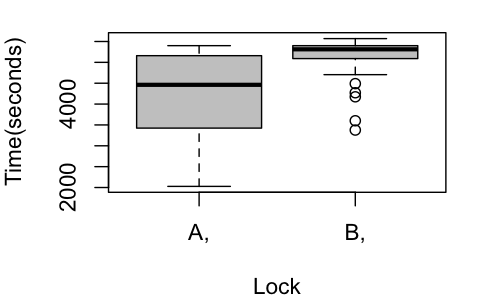
\includegraphics[height=4.5cm]{img/u1.png}
\caption{First experiment box-plot graphic.}
\end{figure}

\begin{figure}
\centering
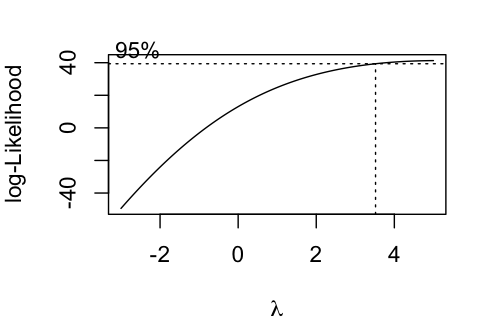
\includegraphics[height=4.5cm]{img/u2.png}
\caption{First experiment box-cox transformation check ($$\lambda = 5$).}
\end{figure}

\begin{figure}
\centering
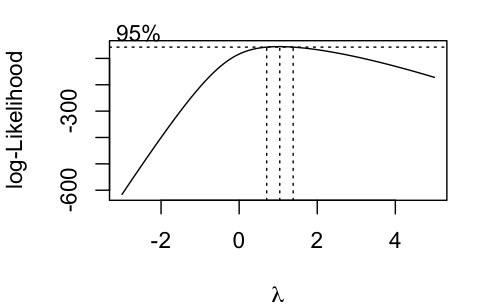
\includegraphics[height=4.5cm]{img/u2boxcox.png}
\caption{First experiment box-cox transformation applied.}
\end{figure}

% Describe undergrad students analysis, put plots generated by R %
% lambda: 5 (apply boxcox transf) %
% tukey: 0.5146133 (after transf) %

\begin{table}
\begin{center}
\caption{Undergraduate students ANOVA results}
\begin{tabular}{|l|l|l|l|l|ll|}
\hline
                & Df &    Sum Sq  &  Mean Sq   & F value & Pr(>F)    &     \\  
replica         & 14 & 3.8633e+37 & 2.7595e+36 & 1.6553  & 0.1784197 &     \\   
program         & 1  & 4.1460e+36 & 4.1460e+36 & 2.4869  & 0.1371197 &     \\   
lock            & 1  & 3.9489e+37 & 3.9489e+37 & 23.6873 & 0.0002492 & *** \\
replica:student & 15 & 4.1013e+37 & 2.7342e+36 & 1.6401  & 0.1808595 &     \\  
replica:lock    & 14 & 2.4033e+37 & 1.7166e+36 & 1.0297  & 0.4785520 &     \\  
Residuals       & 14 & 2.3340e+37 & 1.6671e+36 &         &           &     \\
\hline
\end{tabular}
\end{center}
\end{table}

% Describe grad students analysis, put plots generated by R %
% lambda: 1.3636 (apply boxcox transf) %
% tukey: 0.9141885 (after transf) %

\begin{figure}
\centering
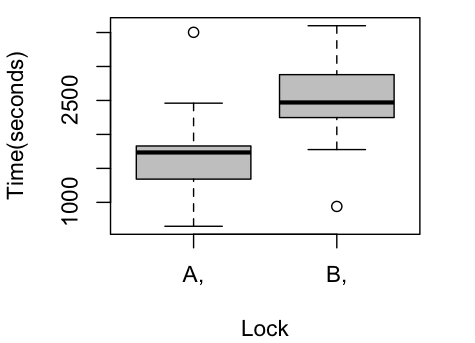
\includegraphics[height=4.5cm]{img/g1.png}
\caption{Second experiment box-plot graphic.}
\end{figure}

\begin{figure}
\centering
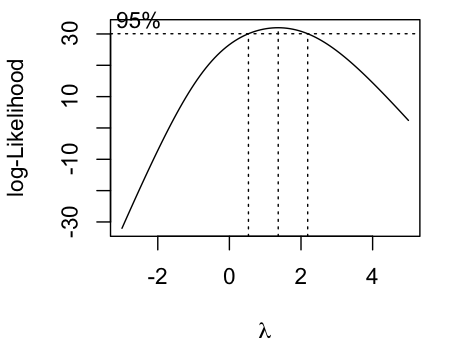
\includegraphics[height=4.5cm]{img/g2.png}
\caption{Second experiment box-cox transformation check ($$\lambda = 1.3636$).}
\end{figure}

\begin{figure}
\centering
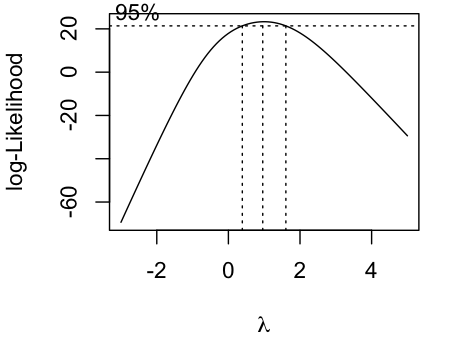
\includegraphics[height=4.5cm]{img/g2boxcox.png}
\caption{Second experiment box-cox transformation applied.}
\end{figure}

\begin{table}
\begin{center}
\caption{Graduate students ANOVA results.}
\begin{tabular}{|l|l|l|l|l|ll|}
\hline
                 & Df &    Sum Sq &   Mean Sq  & F value &   Pr(>F) & \\   
\hline
replica          & 6 & 2576883250 &  429480542 & 14.1891 & 0.0025793 & **  \\
program          & 1 &    6875586 &    6875586 &  0.2272 & 0.6505035 &     \\
lock             & 1 & 1958179433 & 1958179433 & 64.6938 & 0.0001975 & *** \\
replica:student  & 7 & 2328154077 &  332593440 & 10.9881 & 0.0047601 & **  \\
replica:lock     & 6 &  823830276 &  137305046 &  4.5362 & 0.0441188 & *   \\
Residuals        & 6 &  181610625 &   30268438 &         &           &     \\
\hline
\end{tabular}
\end{center}
\end{table}

\emph{2) Accuracy Analysis:} Applying Fisher's exact test we can see that undergraduate students did receive an improvement on accuracy (see Table 2), while graduate students did not have any significant difference for the accuracy (see Table 3).

\begin{table}
\begin{center}
\caption{Undergraduate students results presented a two-tailed P value equals 0.0004. The association between rows (groups) and columns (outcomes) is considered to be extremely statistically significant}
\begin{tabular}{|l|l|l|}
\hline
 & Correct & Incorrect\\
\hline
LockA & 29 & 2\\
LockB & 16 & 15\\
\hline
\end{tabular}
\end{center}
\end{table}

\begin{table}
\begin{center}
\caption{Graduate students results presented a two-tailed P value equals 0.3259. The association between rows (groups) and columns (outcomes) is considered to be not statistically significant}
\begin{tabular}{|l|l|l|}
\hline
 & Correct & Incorrect\\
\hline
LockA & 13 & 1\\
LockB & 10 & 4\\
\hline
\end{tabular}
\end{center}
\end{table}

\subsection{Results Interpretation}

We can see that accuracy was indeed improved for unexperienced subjects but may not have any big impact in more experienced subjects, like we expected. However, both groups did improve time.

We believe that our imposed time limit have limited more drastically the time ranges on the first group because they spent more time on each question. Also the fact it was an exam for them may have delayed the time to answer because they were more careful. We have observed during the experiment that many students wrote their answers but they were reluctant to ask for the next question because they still have plenty of time left and they wanted to make sure it was correct. We did not observe such behavior with the second group of students and we believe it is because they did not have the same pressure to deliver correct results.

\subsection{Threats To Validity}

\dots

% TODO: move this to the end of paper %
% TODO: add instructions for plc students result analysis %
\subsection{Attachments}

\noindent
{\it Instructions in R to evaluate time}
\begin{verbatim}
exp1.dat = read.table(file="/Users/rafaelbrandao/r_input.dat", header = T)
attach(exp1.dat)

replica = factor(replica.)
student = factor(student.)
program = factor(program.)
lock = factor(lock.)

# Plot the box plot graphic using the response variable (time)
# associated with the locks with the following command

plot(time~lock,col="gray",xlab="Lock",ylab="Time(seconds)")

# We set the effect model that will serve as basis for posterior analysis.
# Notice that the factor student is associated with the factor replica since for
# each replica we used a different pair of students. We also included the factor
# lock associated with the replica.

anova.ql<-aov(time~replica+student:replica+program+lock+lock:replica)

library(MASS)
bc <- boxcox(anova.ql,lambda = seq(-3, 5, 1/10))
# If transformation is needed, we calculate lambda and use it:
# anova.ql<-aov(time**<lambda>~replica+student:replica+program+lock+lock:replica)
lambda <- bc$x[which.max(bc$y)]

TukeyNADD.QL.REP<-function(objeto1)
{
y1<-NULL
y2<-NULL
y1<- fitted(objeto1)
y2<- y1^2
objeto2<- aov(y2 ~ objeto1[13]$model[,2] +
objeto1[13]$model[,3]:objeto1[13]$model[,2]
+ objeto1[13]$model[,4]+ objeto1[13]$model[,5])
ynew <- resid(objeto1)
xnew <- resid(objeto2)
objeto3 <- lm(ynew ~ xnew)
M <- anova(objeto3)
MSN <- M[1,3]
MSErr <- M[2,2]/(objeto1[8]$df.residual-1)

F0 <- MSN/MSErr
p.val <- 1 - pf(F0, 1,objeto1[8]$df.residual-1)
p.val
}
TukeyNADD.QL.REP(anova.ql)

plot(anova.ql)
anova(anova.ql)
\end{verbatim}

\noindent
{\it Undergraduate students's time results. Input used in R for analysis}
\begin{verbatim}
replica, student, program, lock, time
1, 1, p1, A, 4996
1, 1, p2, B, 5367
1, 2, p1, B, 5070
1, 2, p2, A, 5260
2, 3, p1, A, 2700
2, 3, p2, B, 5306
2, 4, p1, B, 4490
2, 4, p2, A, 4017
3, 5, p1, A, 2340
3, 5, p2, B, 5290
3, 6, p1, B, 3377
3, 6, p2, A, 4473
4, 7, p1, A, 5400
4, 7, p2, B, 5360
4, 8, p1, B, 5400
4, 8, p2, A, 3641
5, 9, p1, A, 5400
5, 9, p2, B, 5400
5, 10, p1, B, 3600
5, 10, p2, A, 2406
6, 11, p1, A, 3290
6, 11, p2, B, 5370
6, 12, p1, B, 5400
6, 12, p2, A, 5320
7, 13, p1, A, 3424
7, 13, p2, B, 5356
7, 14, p1, B, 5400
7, 14, p2, A, 5160
8, 15, p1, A, 2593
8, 15, p2, B, 5279
8, 16, p1, B, 4705
8, 16, p2, A, 4535
9, 17, p1, A, 5160
9, 17, p2, B, 5430
9, 18, p1, B, 5250
9, 18, p2, A, 4246
10, 19, p1, A, 4967
10, 19, p2, B, 5413
10, 20, p1, B, 5400
10, 20, p2, A, 3804
11, 21, p1, A, 5280
11, 21, p2, B, 5160
11, 22, p1, B, 4174
11, 22, p2, A, 4886
12, 23, p1, A, 4271
12, 23, p2, B, 5569
12, 24, p1, B, 5400
12, 24, p2, A, 4788
13, 25, p1, A, 5400
13, 25, p2, B, 5239
13, 26, p1, B, 5310
13, 26, p2, A, 5390
14, 27, p1, A, 2027
14, 27, p2, B, 4271
14, 28, p1, B, 5090
14, 28, p2, A, 4450
15, 29, p1, A, 3000
15, 29, p2, B, 5315
15, 30, p1, B, 5400
15, 30, p2, A, 4210
\end{verbatim}

\noindent
{\it Graduate students's time results. Input used in R for analysis}
\begin{verbatim}
replica, student, program, lock, time
1, 1, p1, A, 1757
1, 1, p2, B, 2404
1, 2, p1, B, 1777
1, 2, p2, A, 1716
2, 3, p1, A, 1342
2, 3, p2, B, 2552
2, 4, p1, B, 2597
2, 4, p2, A, 1238
3, 5, p1, A, 1572
3, 5, p2, B, 2248
3, 6, p1, B, 3168
3, 6, p2, A, 2460
4, 7, p1, A, 1822
4, 7, p2, B, 2455
4, 8, p1, B, 2486
4, 8, p2, A, 2434
5, 9, p1, A, 3503
5, 9, p2, B, 3600
5, 10, p1, B, 2454
5, 10, p2, A, 1753
6, 11, p1, A, 1830
6, 11, p2, B, 3300
6, 12, p1, B, 2880
6, 12, p2, A, 890
7, 13, p1, A, 648
7, 13, p2, B, 940
7, 14, p1, B, 2247
7, 14, p2, A, 1363
\end{verbatim}
